\documentclass[16pt]{article}
\usepackage[english]{babel}
\usepackage{longtable}
\usepackage[top=1in, bottom=0.25in, left=1.25in, right=1.25in,includefoot,heightrounded]{geometry}
\usepackage{indentfirst}
\usepackage[utf8]{inputenc}
\usepackage{amsmath,amssymb}
\usepackage{graphicx,tikz}
\usepackage{hyperref}
\usepackage[colorinlistoftodos]{todonotes}
\usepackage[document]{ragged2e}
\usepackage{fancyhdr}
\usepackage{enumerate}
\usepackage{listings}
\usepackage{color}
\usepackage{flowchart}
\usepackage{hyperref}
\usepackage{graphicx}
\usetikzlibrary{arrows}


\usetikzlibrary{shapes.geometric, arrows}
\tikzstyle{startstop} = [rectangle, rounded corners, minimum width=3cm, minimum height=1cm,text centered, draw=black, fill=red!30]
\tikzstyle{decision} = [diamond, minimum width=4cm, minimum height=0.5cm, text centered, draw=black, fill=green!30]
\tikzstyle{process} = [rectangle, minimum width=3cm, minimum height=1cm, text centered, draw=black, fill=orange!30]
\tikzstyle{arrow} = [thick,->,>=stealth]
\tikzstyle{io} = [trapezium, trapezium left angle=70, trapezium right angle=110, minimum width=2cm, text width=4cm, minimum height=1cm, text centered, draw=black, fill=blue!30]

\pagestyle{fancy}
\fancyhf{}
\lhead{Myles Deslippe}
\rhead{Comp 3670 | Computer Networks}
\cfoot{\thepage}

\definecolor{MyDarkGreen}{rgb}{0.0,0.4,0.0}
\lstset{inputencoding=ansinew}
\lstset{breaklines=true} 

\begin{document}

    \section*{\centering{Network Applications}}

    \subsection*{Principals of Network Applications}
    \begin{itemize}
        \item To create a \textbf{network application}, we need to write a program that runs on \textbf{different end systems}, and \textbf{communicates over a network}.
        \item There is a \textbf{layer of abstraction} between \textbf{network applications} and \textbf{the network}; allowing for \textbf{rapid network application development}.
        \item There are different \textbf{application architectures} we can use to developer \textbf{network applications}.
    \end{itemize}

    \subsection*{Client-Server Architecture}
    \begin{itemize}
        \item The \textbf{client-server architecture} consists of two entities, the \textbf{client} and the \textbf{server}.
        \item The \textbf{sever} is a \textbf{network host that is always on}, and has a \textbf{permanent IP address}.
        \item The \textbf{client} communicate with the \textbf{server} over a \textbf{network}, and can have a \textbf{dynamic IP address}.
        \item The clients do not \textbf{directly communicate}, they use the \textbf{server to communicate}.
    \end{itemize}

    \subsection*{Peer to Peer Architecture}
    \begin{itemize}
        \item The \textbf{peer to peer architecture} has \textbf{no always-on server}.
        \item The \textbf{clients communicate directly}.
    \end{itemize}

    \subsection*{Process Communication}
    \begin{itemize}
        \item A \textbf{process} is a \textbf{program running on a network host}.
        \item \textbf{Processes} in the \textbf{same host} use \textbf{inter-process communication} to communicate.
        \item \textbf{Processes} in \textbf{different hosts} use \textbf{network-communication} to communicate.
        \item The \textbf{server process} is a process that \textbf{waits to be contacted by clients}.
        \item The \textbf{client process} is a process that \textbf{initiates communication with the server}.
    \end{itemize}

    \subsection*{Sockets}
    \begin{itemize}
        \item One way \textbf{two process} can \textbf{connect over a network} is with \textbf{sockets}.
        \item A \textbf{socket} is a \textbf{structure within a network host} that \textbf{serves as an endpoint} for \textbf{sending and receiving data}.
        \item In order for \textbf{network hosts to communicate}, they must each have a \textbf{unique Internet Protocol Address (IP Address)}.
        \item The \textbf{operating system} uses the \textbf{ports} of the \textbf{server and client} to make sure the information ends up in the \textbf{correct place}.
    \end{itemize}

    \subsection*{Application Layer Protocols}
    \begin{itemize}
        \item \textbf{Application Layer Protocols} define how \textbf{application processes} running on \textbf{different end systems communicate}.
        \item The \textbf{protocols} define \textbf{the message syntax, semantics, and rules}.
        \item The \textbf{type of transport} an \textbf{application} uses depends on what is \textbf{important to the application}; such as \textbf{data integrity, throughput, timing, etc}.
    \end{itemize}

    \subsection*{Internet Transport Services}
    \begin{itemize}
        \item There are \textbf{two internet transport protocol services}:
        \begin{enumerate}
            \item \textbf{User Datagram Protocol (UDP)} is a \textbf{transport protocol} that is \textbf{fast but unreliable}. UDP has \textbf{no confirmation} that the \textbf{packets were delivered}; upd is \textbf{not connection-oriented}.
            \item \textbf{Transport Control Protocol (TCP)} is a \textbf{transport protocol} that is \textbf{reliable, but has more overhead}. TCP has \textbf{flow control, congestion control, and is connection oriented}.
        \end{enumerate}
        \item \textbf{TCP and UDP} have \textbf{no encryption} by default.
        \item To \textbf{secure data} being transferred with \textbf{TCP} we use a \textbf{Secure Socket Layer (SSL)} which provides \textbf{encryption, data integrity, and end-point authentication}.
        \begin{itemize}
            \item \textbf{SSL} is a part of the \textbf{application-layer}.
        \end{itemize}
    \end{itemize}

    \section*{\centering{The World Wide Web}}

    \subsection*{Introduction}
    \begin{itemize}
        \item The \textbf{Word Wide Web or Web} is the world's dominant \textbf{software platform}.
        \item The \textbf{web} is an information space where \textbf{documents and other resources} can be \textbf{accessed through the internet} using a \textbf{web browser}.
        \item A \textbf{web page} is a \textbf{hypertext document} that is delivered by a \textbf{web server}.
        \item A \textbf{website} consists of \textbf{many webpages} linked together under a common \textbf{host}.
        \item \textbf{Web resources} can be accessed through a \textbf{Uniform Resource Locator (URL)}.
        \item[] 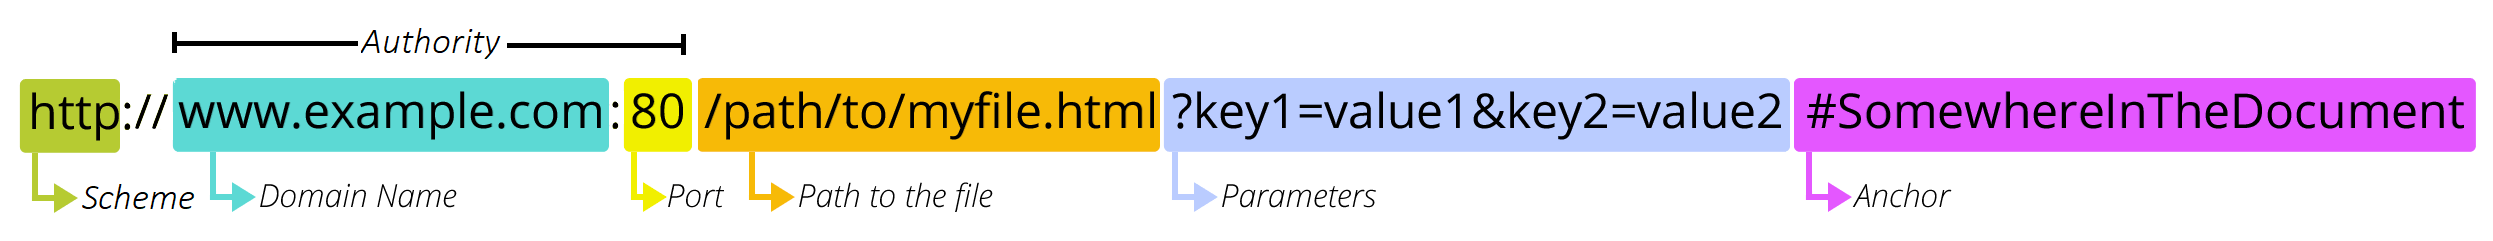
\includegraphics[width=407px]{images/URL.png}
    \end{itemize}
    
    \subsection*{Hypertext Transfer Protocol}
    \begin{itemize}
        \item The \textbf{web} uses the \textbf{Hypertext Transfer Protocol (HTTP) suite} to transfer data over the \textbf{internet}.
            \item \textbf{HTTP} uses \textbf{TCP} to facilitate the actual data transfer as follows:
            \begin{enumerate}
                \item The \textbf{client} initiates the \textbf{TCP} connection with the \textbf{server} (typically on port 80).
                \item The \textbf{server} accepts the \textbf{TCP} connection from the \textbf{client}.
                \item \textbf{HTTP messages} are exchanged between the \textbf{browser} and the \textbf{server}.
                \item The \textbf{TCP} connection is \textbf{closed}.
            \end{enumerate}
        \item \textbf{HTTP} is \textbf{stateless}.
        \item There are \textbf{two} types of \textbf{HTTP connections}:
        \begin{enumerate}
            \item \textbf{Persistent HTTP} is a connection where multiple files can be sent over a \textbf{single TCP connection} between the \textbf{client} and the \textbf{server}.
            \item \textbf{Non-Persistent HTTP} is where each file requires a \textbf{separate TCP connection} between the \textbf{client} and the \textbf{server}. 
        \end{enumerate}

    \end{itemize}

    \subsection*{Hypertext Transfer Protocol Versions}
    \begin{itemize}
        \item \textbf{HTTP 1.0} key features:
        \begin{enumerate}
            \item The concept of headers and request methods were introduced.
            \item Version information is include in requests.
            \item It allowed for a single request / response for every TCP connection.
            \item Status codes were introduced.
            \item The content-type header made it possible to send different file types.
        \end{enumerate}
        \item \textbf{HTTP 1.1} key features:
        \begin{enumerate}
            \item Allows for multiple requests with a single TCP connection via the keep-alive header.
            \item The upgrade header was introduced to allow the server and the client to switch communication protocols.
            \item Support for chunk transfers was introduced allowing for streaming content dynamically.
        \end{enumerate}
        \item \textbf{HTTP 2.0} key features:
        \begin{enumerate}
            \item The protocol has switched to a binary protocol (no more plain text requests).
            \item Introduced push servers, allowing the server to push common resources before the client requests them.
            \item Introduced multiplexing interleaving the requests and responses without head-of-line blocking over a single TCP connection.
        \end{enumerate}
    \end{itemize}

    \subsection*{Hypertext Transfer Protocol Requests}
    \begin{itemize}
        \item \textbf{HTTP requests} are the \textbf{messages} used to communicate over the \textbf{HTTP protocol}.
        \item There are \textbf{two main parts} of the request:
        \begin{enumerate}
            \item \textbf{The Header} is the field of an \textbf{HTTP request or response} that passes \textbf{additional context and metadata} about the request.
            \item \textbf{The Body} is the field of an \textbf{HTTP request or response} that passes the \textbf{target data}.
        \end{enumerate}
        \item There are two \textbf{8 types of HTTP request methods}:
        \begin{enumerate}
            \item The \textbf{GET method} is used to \textbf{retrieve information} from the server.
            \item The \textbf{HEAD method} is used to \textbf{retrieve information} from the server, but it transfers the status line and the header only.
            \item The \textbf{POST method} is used to \textbf{send data} to the server.
            \item The \textbf{PUT method} is used to \textbf{replace data} on the server.
            \item The \textbf{DELETE method} is used to \textbf{delete data} on the server.
            \item The \textbf{CONNECT method} is used to \textbf{establish a tunnel to the server}.
            \item The \textbf{OPTIONS method} is used to \textbf{describe the communication options} for the target resource.
            \item The \textbf{TRACE method} is used to \textbf{perform a message loop back test}.
        \end{enumerate}
    \end{itemize}
    
    \subsection*{Maintaining State over HTTP}
    \begin{itemize}
        \item Since \textbf{HTTP requests have no state}, we use \textbf{cookies}.
        \item \textbf{Cookies} are \textbf{key-value pairs} that are \textbf{sent back-and-forth with each request} (similar to headers).
    \end{itemize}

    \subsection*{Web Cache (Proxy Servers)}
    \begin{itemize}
        \item ISPs will use \textbf{cache proxy servers} to serve \textbf{cached data}, to lessen the load on the \textbf{origin server}.
        \item If the data is \textbf{not found on the cache proxy server}, the request will be \textbf{forwarded to the origin server}.
        \item \textbf{Cache servers} can reduce the response time for requests, and reduce the traffic on access links.
        \item A \textbf{conditional GET} request is a request that uses the \textbf{cached resource} if it is \textbf{up-to-date}. This uses the \textbf{If-modified-since} header.
    \end{itemize}

    \section*{\centering{Electronic Main}}

    \subsection*{E-Mail Components}
    \begin{itemize}
        \item There are \textbf{three components} to e-mail:
        \begin{enumerate}
            \item \textbf{User Agents} - Software that \textbf{acts on behalf of a user} (composing, editing, sending, and displaying email messages).
            \item \textbf{Mail Servers} - Software that \textbf{transfers electronic mail}.
            \item \textbf{Simple Mail Transfer Protocol (SMTP)} - An \textbf{internet standard} for communicating \textbf{electronic mail}.
        \end{enumerate}
        \item A \textbf{mailbox} is a container that \textbf{store incoming messages} for the user.
        \item The \textbf{message queue} is a queue of \textbf{outgoing messages}.
        \item \textbf{SMTP} facilitates the \textbf{transfer of messages}.
    \end{itemize}

    \subsection*{Simple Mail Transfer Protocol (SMTP)}
    \begin{itemize}
        \item \textbf{Simple Mail Transfer Protocol} uses the \textbf{TCP protocol} to reliably \textbf{transfer email messages} from the client to the server.
        \item \textbf{Unencrypted mail} typically uses \textbf{port 25}.
        \item There are \textbf{three phases of transfer}:
        \begin{enumerate}
            \item The handshake phase.
            \item The message transfer phase.
            \item The closure phase.s
        \end{enumerate}
        \item \textbf{Commands} use ASCII text, and \textbf{responses} use status codes and phrases.
        \item \textbf{Messages} must be in \textbf{7-bit ASCII}.
        \item \textbf{Messages} have a \textbf{header} and a \textbf{body}.
    \end{itemize}

    \subsection*{Mail Access Protocols}
    \begin{itemize}
        \item \textbf{Simple Mail Transfer Protocol (SMTP)} is a protocol that allows email clients to \textbf{deliver and store} messages on a \textbf{receiver's} server.
        \item \textbf{Internet Mail Access Protocol (IMAP)} is a protocol that allows email clients to \textbf{retrieve, delete, and store} messages on a mail server.
        \item \textbf{Hypertext Transfer Protocol (HTTP)} can be used to create a \textbf{web-interface} on top of \textbf{SMTP and IMAP}.
    \end{itemize}

    \section*{\centering{Domain Name System}}

    \subsection*{Domain Name System}
    \begin{itemize}
        \item The \textbf{Domain Name System (DNS)} is a \textbf{hierarchial} and \textbf{decentralized naming system} that is used to \textbf{identify computers} that are reachable over the \textbf{internet}.
        \item A \textbf{name server} is a single \textbf{server component} of the \textbf{domain name system}.
        \item The \textbf{DNS} allows computers to translate \textbf{domains} (ex google.com) to \textbf{IP addresses}. 
    \end{itemize}

    \subsection*{DNS Root Name Servers}
    \begin{itemize}
        \item \textbf{DNS root servers} are official, contact-of-last-resort servers that \textbf{cannot resolve names}. They are managed by the \textbf{Internet Corporation for Assigned Names and Numbers (ICANN)}.
        \item \textbf{DNS root servers} can direct requests to \textbf{Top-Level Domain (TLD) servers}.
        \item The internet \textbf{would not work} without \textbf{root servers}.
        \item \textbf{DNSSEC} is used to provide \textbf{DNS security} (authentication and message integrity).
    \end{itemize}

    \subsection*{Top-Level Domain Servers}
    \begin{itemize}
        \item \textbf{Top-Level Domain servers} are servers that are responsible for .com, .org, .net, .ca, etc.
        \item \textbf{Authoritative DNS servers} are \textbf{DNS servers} that are owned by \textbf{organizations}, and provide \textbf{authoritative hostname to IP mappings} for organizations named hosts.
    \end{itemize}

    \subsection*{Local DNS Servers}
    \begin{itemize}
        \item \textbf{Local DNS servers} are \textbf{DNS servers} that are owned and operated by \textbf{internet service provides, companies, and universities}.
        \item When you make a \textbf{DNS request}, it goes to your \textbf{local DNS server}, if your \textbf{local DNS server does not have the mapping}, it will act as a proxy up the \textbf{DNS} hierarchy.
    \end{itemize}

    \subsection*{DNS Hierarchy}
    \begin{itemize}
        \item[] 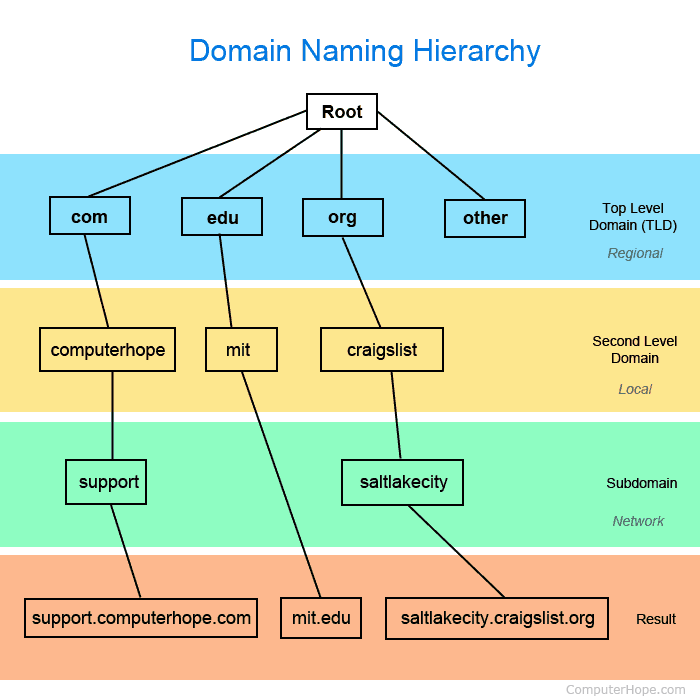
\includegraphics[width=407px]{images/DNS.png}
    \end{itemize}

    \subsection*{Types of DNS Name Resolution}
    \begin{itemize}
        \item There are \textbf{two types} of \textbf{DNS name resolution}:
        \begin{enumerate}
            \item \textbf{Iterated query} is where the \textbf{local DNS server contacts other DNS servers}, and \textbf{if the server cannot resolve the domain} the other DNS server \textbf{redirect the local DNS server}. This process continues until the \textbf{domain is resolved, or it is discovered that the domain does not exist}.
            \item \textbf{Recursive query} is where the \textbf{local DNS server contacts one DNS server}, if the DNS server \textbf{cannot resolve the domain, it will forward the request}. This process continues until the \textbf{domain is resolved, or it is discovered that the domain does not exist}.
        \end{enumerate}
        \item \textbf{Iterated queries} put a \textbf{heavy-load} on \textbf{local DNS servers}.
        \item \textbf{Recursive queries} put a \textbf{heavy-load} on \textbf{non-local DNS servers}.
        \item With \textbf{recursive queries} each time a new \textbf{domain is resolved} it can be \textbf{cached} on \textbf{all of the servers} that \textbf{forwarded the request}, whereas with \textbf{iterative queries} it will \textbf{only be cached on the local DNS server}.
    \end{itemize}

    \subsection*{DNS Caching and Updating}
    \begin{itemize}
        \item One a \textbf{name server} learns a \textbf{mapping}, it \textbf{caches the mapping}.
        \item Each \textbf{cached entry} has a \textbf{timeout period (Time To Live | TTL)}. The TTL can be defined when setting up the domain.
        \item \textbf{Cached entries} may be \textbf{out-of-date} since they are only updated when the mapping \textbf{times out}.
        \item The delay it takes for of the \textbf{DNS servers} to update their \textbf{DNS mapping} is known as \textbf{propagation delay}.
    \end{itemize}

    \subsection*{Types of DNS Records}
    \begin{itemize}
        \item \textbf{DNS records (RR records)} are stored with the following format: \textbf{(name, value, type, ttl)}.
        \item An \textbf{A Record} is an \textbf{IPv4 address mapping record (or DNS host record)}. It stores a \textbf{hostname} and it's corresponding \textbf{IPv4 address}.
        \item An \textbf{AAAA Record} is an \textbf{IPv6 address mapping record (or DNS host record)}. It stores a \textbf{hostname} and it's corresponding \textbf{IPv6 address}.
        \item A \textbf{Canonical Name Record (CNAME Record)} is a record to \textbf{alias hostnames}. It stores a \textbf{from hostname} and a \textbf{to hostname}.
        \item A \textbf{Mail Exchanger Record (MX Record)} is a record to specify a \textbf{SMTP email server} for the domain. It is used to \textbf{route outgoing} emails to an \textbf{email server}.
        \item A \textbf{Name Server Record (NS Record)} is a record that indicates a \textbf{DNS Zone} is \textbf{delegated to an Authoritative Name Server}, and provides the \textbf{address of the name server}.
        \item A \textbf{Reverse-Lookup Pointer Record (PTR Record)} allows a \textbf{DNS resolver} to provides an \textbf{IP address} and \textbf{receives a hostname} (Reverse DNS lookup).
        \item A \textbf{Certificate Record (CERT Record)} is a record that stores encryption certificates (PKIX, SPKI, PGP, etc).
        \item A \textbf{Service Location Record (SRV Record)} is a record that \textbf{specifies a service location} (similar to MX Records, but for other communication protocols).
        \item A \textbf{Text Record (TXT Record)} is a record that \textbf{carries machine-readable data} (DKIM, DMARC, sender policy, etc).
        \item A \textbf{State of Authority Record (SOA Record)} is a record that \textbf{appears at the beginning of a DNS zone file}. It is used to indicate the \textbf{authoritative name server} for the current \textbf{DNS zone}. Contact information for the domain administrator, and other meta-data is stored here.
    \end{itemize}

    \subsection*{DNS Protocol Messages}
    \begin{itemize}
        \item \textbf{DNS query and reply} messages \textbf{have the same format}:
        \item[] 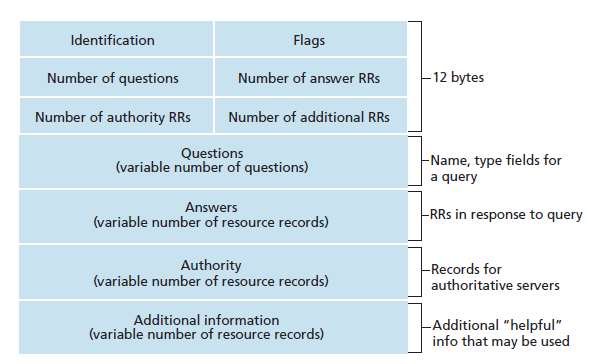
\includegraphics[width=407px]{images/DNS-Message.png}
        \begin{itemize}
            \item \textbf{Identification} is a \textbf{16-bit integer}, the \textbf{reply will respond with the same number}.
            \item \textbf{Flags} are: query or reply, recursion desired, recursion available, reply is authoritative.
        \end{itemize}        
    \end{itemize}

    \section*{\centering{Socket Programming}}

    \subsection*{Sockets}
    \begin{itemize}
        \item A \textbf{socket} is a \textbf{communication endpoint} that hosts use to \textbf{communicate}.
        \item \textbf{Socket programming} is the process of \textbf{creating programs} that use \textbf{sockets} to \textbf{communicate}.
    \end{itemize}

    \subsection*{Types of Socket Programming}
    \begin{itemize}
        \item There are two types of socket programming:
        \begin{enumerate}
            \item \textbf{User Datagram Protocol (UDP)} | UDP is a protocol that \textbf{does not have a handshake} before data is exchanged. The sender may attempt to transmit data, but there is no confirmation that it was, or was not recieved.
            \item \textbf{Transmission Control Protocol (TCP)} | TCP is a protocol that enables communication between a \textbf{client} and a \textbf{server}. Before the connection can be established, the \textbf{server} must be running with a socket. \textbf{Clients} can then connect to that socket, with their own socket. TCP has a \textbf{handshake} before messages are exchanged, and \textbf{ensures message delivery}.
        \end{enumerate}
    \end{itemize}

\end{document}